\documentclass[11pt,a4paper]{article}
\usepackage[latin1]{inputenc}
% \usepackage[swedish]{babel} % s�tt ett % framf�r denna rad om du skriver p� engelska
\usepackage{amsmath}
\usepackage{graphicx}
\usepackage{amssymb}
\usepackage{xcolor}  
\usepackage{enumitem}
\usepackage{booktabs}
\usepackage{float}

\usepackage[colorlinks=true, breaklinks=true]{hyperref}
\usepackage[backend=biber,style=authoryear]{biblatex}
\addbibresource{references.bib}


\title{To be determined) }
\author{Emilio Otero Johansson}


%%%%%%%%%%%%%%%%%%%%%%%%%%%%%%%%%%%%%%%%%%%%%%%%%%%%%%%
\begin{document} % H�r b�rjar den egentliga texten
%%%%%%%%%%%%%%%%%%%%%%%%%%%%%%%%%%%%%%%%%%%%%%%%%%%%%%%


\begin{abstract}
Accurate estimation of population age structure is important in wildlife ecology, but age is often measured with error. This thesis studies how to recover a latent age distribution from misclassified observations using statistical deconvolution in a simulation setting. The true population structure is generated from a Leslie matrix model, while measurement error is introduced through a misclassification mechanism.

Two estimators are evaluated: a method-of-moments (MoM) estimator and a maximum likelihood estimator implemented via the Expectation--Maximization (EM) algorithm. Their performance is assessed through Monte Carlo simulations under different levels of measurement error and sample size, using total variation distance and population forecasts. Results are compared to an oracle baseline and to the naive estimator based on misclassified observations.

The results show that under ill-posed conditions the EM estimator reduces bias but has higher variability, while the naive estimator and MoM are more stable but systematically biased. The study shows that even small bias in age structure can lead to large errors in population forecasts, highlighting that improvements in statistical performance do not necessarily translate into improved ecological performance.
\end{abstract}

\tableofcontents

\section{Introduktion}\label{stycke1}


Accurate knowledge of population structure is fundamental in wildlife ecology, particularly for long-lived species where survival and reproduction vary strongly with age. In Scandinavian brown bear populations, age composition plays a central role in understanding population growth, reproductive potential, and long-term sustainability. For this reason, monitoring programs, such as the Swedish Environmental Protection Agency?s national wildlife monitoring scheme, regularly collect biological data to estimate population size and structure, including age distributions of bears \cite{nrm_bear_monitoring}.

A central challenge in such monitoring efforts is that age is rarely observed directly. Instead, age is typically inferred using indirect biological indicators such as tooth cementum layers or other morphological measurements. These procedures are inherently subject to measurement uncertainty and classification error. As a result, the observed age distribution does not perfectly reflect the true underlying population structure. This discrepancy can introduce bias into demographic estimates and may propagate into downstream analyses such as population forecasting and management decisions.

A recent development in biological indicators used for age determination is the work by Nakamura et al. \cite{nakamura2023}, who propose an age estimation method for brown bears based on blood DNA methylation levels. This approach provides a molecular alternative to traditional age determination techniques, which are often based on tooth wear or cementum annuli. While such methods can improve individual-level age estimation, they still produce observations that are subject to measurement error and uncertainty, which propagates into population-level age structure estimates.

In general, any age estimation method introduces a stochastic relationship between the true age and the observed measurement. This motivates statistical approaches that explicitly model the meassurment error and its relationship to the true age distribution. Such approache can be formulated as a deconvolution problem, where the observed data are viewed as a convolution of the true age distribution and a measurement error mechanism. The effectiveness of these methods depends on both the severity of measurement error and the amount of available data.

The present thesis investigates this deconvolution problem in a controlled simulation setting. The true population age structure is generated using a Leslie matrix model, which provides a biologically grounded age-dependent population dynamic. Measurement error is then introduced through a probabilistic misclassification mechanism, producing an observed age distribution that deviates from the latent structure.

The main objective of this study is to evaluate how well the latent age distribution can be recovered using a deconvolution approach based on the Expectation-Maximization (EM) algorithm and method-of-moments (MoM). In particular, the performance of the method is assessed under two different levels of measurement error and five different sample sizes. The quality of the estimated distributions is evaluated using total variation distance, while the practical implications of estimation error are further examined through population forecasting using the Leslie matrix model.

By combining a structured demographic model with a controlled measurement error framework, this study aims to provide insight into the conditions under which deconvolution methods can meaningfully improve inference about population age structure, and when such corrections may or may not translate into improved ecological forecasts.

\section{Methodology}\label{stycke2}

\subsection{Deconvolution}\label{sec:deconvolution}

Measurement error in statistical models can be described as the discrepancy between a latent (true) variable and its observed counterpart. A common way to formalize this is through a convolution structure, where the observed variable is a noisy transformation of the true signal.

\[
Y = Z + \epsilon.
\]

Here, $Z$ denotes the latent random variable, $\epsilon$ denotes measurement error, and $Y$ denotes the observed random variable. The distribution of $Y$ is then the convolution of the distributions of $Z$ and $\epsilon$.

This formulation extends naturally to multivariate settings, where both the latent and observed quantities are represented as random vectors.

\[
\mathbf{Y} = \mathbf{Z} + \mathbf{\epsilon}.
\]

In many applications, including the present one, the variable of interest is discrete. In such cases, the additive error formulation is replaced by a discrete measurement error mechanism, which will be specified in the following sections.

In a deconvolution problem, the goal is to recover the distribution of the latent variable based on observations of the corresponding noisy measurements and under the assumption that the distribution of the error term is fully known. Deconvolution problems are typically ill-posed in the sense that small perturbations in the observed data can lead to large changes in the estimated distribution (e.g.\ due to sampling variation).

\paragraph{Latent distribution}
In this study, the true age structure of the bear population is represented by the parameter vector

 \begin{equation}
 \boldsymbol{\pi} = (\pi_1, \pi_2, \dots, \pi_k), 
 \end{equation} \label{eq:latent_age_dist}
 
 where $\pi_j$ denotes the probability that an individual belongs to age class $j$. In particular, $\pi_1$ corresponds to the age group 0--1 years, $\pi_2$ to 1--2 years, and so on. The discretization of age into fixed classes is also consistent with population structure is often analyzed in biologically meaningful age intervals, where demographic processes such as survival and reproduction are age-class dependent as seen in \cite{nina_bearmodel}. 
 
Let $n$ denote the number of independent individuals in the sample. For each individual $r = 1,\dots,n$, let $Z_r \in \{1,\dots,k\}$ denote the true age class. We assume that the latent age classes are independent and identically distributed with

\[
P(Z_r = j) = \pi_j.
\]

The vector of observed class counts is then defined as

\[
\boldsymbol{Z} = \left(Z_1^{(c)}, Z_2^{(c)}, \dots, Z_k^{(c)}\right),
\]

where

\[
Z_j^{(c)} = \sum_{r=1}^{n} \boldsymbol{1}(Z_r = j)
\]

denotes the number of individuals in age class $j$. It follows that

\[
\boldsymbol{Z} \sim \text{Multinomial}(n, \boldsymbol{\pi}).
\]

\paragraph{Measurement error}\label{par:measurement-error}

As mentioned in section \ref{sec:deconvolution} the measurement error is assumed to be fully known. In this simulation study, we assume a normal distribution for the error term as a simple and tractable way to control the variability in the observations and to introduce systematic measurement error. While this choice may not exactly reflect the error structure described in \cite{nakamura2023}, the aim of this thesis is to investigate the recovery of the latent distribution under a simplified but comparable error setting.

Additionally, we assume that the measurement error depends on the true age class $Z_r$. Specifically, we model
\[
\epsilon_r \mid Z_r=j \sim \mathcal{N}(0, \sigma^2).
\]
Applying the measurement error directly at the individual level would yield a continuous latent measurement $Z_r + \epsilon_r$, which is incompatible with the discrete age-class structure of the model. We therefore define a discrete observation mechanism induced by this continuous error model by discretizing the conditional distribution of $\epsilon_r \mid Z_r = j$ over the $k$ predefined age classes.

Let the probabilities $M_{ij}$ denote the probability of misclassifying a bear of true age j with age i:

\[
M_{ij} = P(Y_r = i \mid Z_r = j)
\] 

Where $Y_r \in \{1,\dots,k\}$ denotes the observed (possibly misclassified) age class corresponding to individual $r$ such that:
\[
\sum_{i = 1}^{k} M_{ij} = 1
\]

This leads to the construction of a square missclassification matrix M with $k$ rows and columns. Representing observed age class $i$ and true age $j$ respectively.

\paragraph{Observed data} \label{par:observed_dist}

Given the misclassification mechanism described above, each individual $r$ with true age class $j$ is observed in age class $i$ with probability $M_{ij}$. Consequently, the observed counts $\mathbf{Y} = (Y_1, \dots, Y_k)$ follow a multinomial distribution with probabilities given by the transformed latent distribution:

\begin{equation}
\mathbf{Y} \sim \text{Multinomial}(n, M \boldsymbol{\pi}).
\label{eq:observed_distribution}
\end{equation}
\paragraph{Naive estimator}

The objective of this thesis is to investigate how well the true age distribution $\boldsymbol{\pi}$ can be recovered from misclassified observations. In the absence of measurement error, a natural estimator of $\boldsymbol{\pi}$ is given by the empirical proportions

\begin{equation}
	\hat{\boldsymbol{\pi}} = \frac{\mathbf{Z}}{n}
	\label{eq:naive_estimate}
\end{equation}

which satisfies $\mathbb{E}[\hat{\boldsymbol{\pi}}] = \boldsymbol{\pi}$.

However, in the presence of measurement error, we observe $\mathbf{Y}$ instead of $\mathbf{Z}$, and the naive estimator $\mathbf{Y}/n$ is generally biased for $\boldsymbol{\pi}$. This motivates the deconvolution approach considered in this thesis.


\subsection{Estimation methods}

In this thesis, we consider two methods for estimating the latent age structure $\boldsymbol{\pi}$: a method-of-moments (MoM) estimator and a maximum likelihood estimator based on the EM algorithm.


\subsubsection{Method of Moments}

The method-of-moments assumes that population moments, such as $\mathbb{E}[\mathbf{Z}]$, can be expressed as functions of the unknown parameter $\boldsymbol{\pi}$. Parameter estimates are obtained by equating these theoretical moments with their empirical counterparts \cite[p.~275]{AlmBritton2008}. 

From equation~\eqref{eq:observed_distribution}, the first moment of the observed data is given by
\begin{equation}
	\mathbb{E}[\boldsymbol{Y}] = n M \boldsymbol{\pi}.
	\label{eq:mom_expectation}
\end{equation}

The corresponding empirical moment is given by the observed proportions $\boldsymbol{Y}/n$ see equation~\ref{eq:naive_estimate}. Equating theoretical and empirical moments yields
\begin{equation}
	M \boldsymbol{\pi} = \frac{\boldsymbol{Y}}{n}.
	\label{eq:mom_equation}
\end{equation}

Solving for $\boldsymbol{\pi}$ gives the MoM estimator
\begin{equation}
	\hat{\boldsymbol{\pi}} = M^{-1} \frac{\boldsymbol{Y}}{n},
\end{equation}
provided that $M$ is invertible.



\paragraph{Matrix regularization}

In practice, the misclassification matrix $M$ may be nearly singular, which makes direct inversion numerically unstable. To address this issue, we apply Tikhonov regularization (ridge regularization), which stabilizes the inversion by penalizing large fluctuations in the estimated parameter vector.

The regularized estimator is defined as
\begin{equation}
	\hat{\boldsymbol{\pi}} =
	\left(M^\top M + \lambda I\right)^{-1} M^\top \frac{\mathbf{Y}}{n},
\end{equation}
where $\lambda > 0$ is a tuning parameter controlling the strength of regularization and $I$ denotes the identity matrix.

The resulting estimator can be written as a linear operator applied to the observed data, 
\[
\hat{\boldsymbol{\pi}} = A_\lambda \frac{\mathbf{Y}}{n},
\]
where
\[
A_\lambda = \left(M^\top M + \lambda I\right)^{-1} M^\top.
\]

\subsubsection{Maximum-likelihood method ML} \label{sec:ML}


The ML method method for parameter estimate consist of arg maxing the log likelihood function for a parameter. Which in our current multinomial case coinced with the estimate for the MoM thus leading to the same problem of matrix inversion (negative estiamtes , probabilities not summing to one). We therfore utilize the Expectation-Maximization algorithm.

\paragraph{Expectation-Maximization (EM) algorithm}
The EM algorithm is a general-purpose method for computing maximum likelihood estimates in the presence of incomplete or latent data (\cite{mclachlan2008}). Let $\boldsymbol{Y}$ denote a discrete random vector corresponding to the observed (incomplete) data, and $\boldsymbol{Z} $ a discrete random vector representing the latent data. Then $\boldsymbol{X}=(\boldsymbol{Y},\boldsymbol{Z})$ is the random vector of the complete data. If $\mathbf{X}$ were fully observable, we could directly compute the complete-data log-likelihood function $\ell_c(\boldsymbol{\pi})$ based on a realization $x$ and estimate $\boldsymbol{\pi}$ by maximum likelihood.

However, in practice we only observe $y \in \mathcal{Y}$. Thus, the EM algorithm considers expectation with respect to the conditional distribution of $\boldsymbol{Z} \mid \boldsymbol{Y}$ and a current parameter estimate $\boldsymbol{\pi}^{(t)}$ \cite{mclachlan2008}:

\begin{equation}
	Q(\boldsymbol{\pi} \mid \boldsymbol{\pi}^{(t)}) = \mathbb{E}_{\boldsymbol{\pi}^{(t)}} \big[ \ell_c(\boldsymbol{\pi}) \mid Y = y \big]
	\label{eq:Qfunction}
\end{equation}


this corresponds to the Expectation step (E-step) of the EM algorithm. In the Maximization step (M-step), the parameter is updated by maximizing this function:

\begin{equation}
	\mathbf{\pi}^{(t+1)} = \arg\max_{\mathbf{\pi}} Q(\mathbf{\pi} \mid \mathbf{\pi}^{(t)}).
	\label{eq:arg_max}
\end{equation}

The process is then iterated upon until $\ell(\mathbf{\pi}^{(t+1)}) - \ell(\mathbf{\pi}^{(t)}) <=  k$ for some arbitrary small $k$ value, which is then interpreted as a local/global maxima.

\paragraph{Monotonicity}. A key property for the algorithm to work is for the likelihood to be monotonically increasing for each iteration. $L(\pi^{(t+1)})\geq L(\pi^{(t)}))$ which is discussed in Section 3.2 of \cite{mclachlan2008}.   



\paragraph{Applying EM-alg}

In principle, the complete data could be represented by individual-level pairs $X = (Z, Y)$, where $Z$ denotes the true age class and $Y$ the observed age class for each individual. With a joint probability function $p_{Z,Y}$ However, in the present multinomial setting it is convenient to work with $N_{ij}$, where $N_{ij}$ denotes the number of individuals with true age class $j$ that are observed in age class $i$. 
 
The joint distribution of true and observed age classes is given by
\begin{equation}
	P(Z=j, Y=i) = \pi_j M_{ij}.
\end{equation}

where $M$ is the misclasification matrix defined in \ref{par:measurement-error} and for a vector of $n$ independent observations  $x_v = {(z_1,y_1),(z_2,y_2),...,(z_n,y_n)}$ we obtain

\begin{equation}
	p_X(x_v;\boldsymbol{\pi}) = \prod_i \prod_j (\pi_j M_{ij})^{n_{ij}}
\end{equation}

where $n_{ij} = \sum_{n=1}1\{Z_r = j , Y_r =i\}$ is a random variable with the counts that were observed as $i$ given they were $j$.

The log-likelihood is then: 

\begin{equation}
	\ell_c(\boldsymbol{\pi}) =  \sum_{j} \sum_{i} n_{ij} \log (p_j M_{ij}) = \sum_{j} \sum_{i} n_{ij} \log  M_{ij} + \sum_{j} \sum_{i} n_{ij} \log \pi_j 
	\label{eq:decomp_likelihood}
\end{equation}

In accordance with equation \eqref{eq:Qfunction} we take the conditional expectation on $n_{ij}$ with an initial parameter $\boldsymbol{\pi^{(0)}}$ conditioned on $Y$ 


\begin{align}
	\mathbb{E}_{\boldsymbol{\pi}^{(0)}} \big[ \ell_c(\boldsymbol{\pi}) \mid \mathbf{Y} = \mathbf{y} \big]
	&=
	\mathbf{E}_{\boldsymbol{\pi}^{(0)}} \Big[ \sum_{j} \sum_{i} n_{ij} \log (\pi_j M_{ij}) \,\Big|\, \mathbf{Y} = \mathbf{y} \Big] \\
	&=
	\sum_{i} \sum_{j} \mathbf{E}_{\boldsymbol{\pi}^{(0)}} \big[n_{ij} \mid \mathbf{Y} = \mathbf{y}\big] \log (\pi_j M_{ij})
\end{align}

The conditional expectation $E_{\boldsymbol{\pi^{(0)}}}[n_{ij} \mid \mathbf{Y} = \mathbf{y}]$ is the expected number of bears with true age class $j$ that are observed in age class $i$, given the observed data $\mathbf{Y} = \mathbf{y}$. Note that this depends on the assumed latent age distribution $\boldsymbol{\pi^{(0)}}$.

Let $Y_i^{(c)}$ denote the number of observed individuals in age class $i$:
\begin{equation}
	Y_i^{(c)} = \sum_{r=1}^{n} \mathbf{1}\{Y_r = i\}
\end{equation}

The expected number of individuals with true age class $j$, among those observed in age class $i$, is given by the number of observed individuals $Y_i^{(c)}$ multiplied by the probability of originating from true age class $j$ given observation in class $i$, $P(Z=j \mid Y=i, \boldsymbol{\pi}^{(0)})$. This probability is proportional to the product of the misclassification probability $M_{ij}$ and the assumed true proportion $\pi_j^{(0)}$, and is normalized by the total probability of being observed in class $i$ from any true age class.

\[
P(Z=j \mid Y=i, \boldsymbol{\pi}^{(0)}) =
\frac{\pi_j^{(0)} M_{ij}}{\sum_{a=1}^{k} \pi_a^{(0)} M_{ia}}
\]


Thus:
\begin{equation}
	\mathbb{E}[n_{ij} \mid Y = y]
	=
	n_j \cdot
	\frac{
		\pi_j^{(0)} M_{ij}
	}{
		\sum_{i'} \pi_{i}^{(0)} M_{ij}
	}
\end{equation}


\paragraph{Maximization-step}

We now choose $\boldsymbol{\pi}^{(t+1)}$ such that, in accordance with equation~\ref{eq:arg_max}, the conditional expected log-likelihood is maximized. From equation~\ref{eq:decomp_likelihood}, we note that only the terms involving $\boldsymbol{\pi}$ depend on the parameter. Thus, the problem reduces to maximizing
\[
\sum_{j} \mathbb{E}[n_{ij} \mid \mathbf{Y} = \mathbf{y}] \, \log \pi_j,
\]
subject to the constraints
\[
\sum_{j} \pi_j = 1, \quad 0 \le \pi_j \le 1.
\]

From Theorem 14.5 (p. 235) in \cite{wasserman2004}, the maximum likelihood estimator for a multinomial random vector $\mathbf{Z} \sim \text{Multinomial}(n, \boldsymbol{\pi})$ is obtained by maximizing
\[
\ell(\boldsymbol{\pi}) = \sum_{j=1}^{k} Z_j \log \pi_j,
\]
under the constraint $\sum_j \pi_j = 1$. Using Lagrange multipliers yields the well-known result
\[
\hat{\pi}_j = \frac{Z_j}{n}, \quad j = 1,\dots,k.
\]

We now replace the unobserved counts $Z_j$ with their conditional expectations
\[
\mathbb{E}[n_{ij} \mid \mathbf{Y} = \mathbf{y}],
\]
which yields the M-step update

\begin{equation}
\pi_j^{(t+1)} =
\cdot
\frac{
	\pi_j^{(t)} M_{ij}
}{
	\sum_{i} \pi_{i}^{(t)} M_{ij}
}
\label{eq:maximization_setp}
\end{equation}


\subsection{Matrix population models}\label{sec:pop_model_matrix}

Matrix population models are a standard framework in population ecology \cite{caswell2001}. In this section, we describe the theoretical framework used to construct a hypothetical true age distribution, which serves as the basis for the simulated data used to evaluate the deconvolution methods considered in this thesis.

\subsubsection{Leslie Matrix}\label{sec:Leslie_Matrix}

To describe the population age structure, we use a matrix population model. Let $j = 1,2,\dots,k$ denote discrete age classes obtained by partitioning a continuous age variable $z$, such that $j-1 \leq z \leq j$.

The population at time $t$ is represented by the vector
\[
\mathbf{v}_t = (n_1, n_2, \dots, n_k),
\]
where $n_j$ denotes the number of individuals in age class $j$.

Let $f_j$ denote the per-capita fertility rate of individuals in age class $j$, defined as the expected number of offspring produced per time step per individual. The total number of offspring produced by age class $j$ is then $n_j f_j$.

In matrix form, the population dynamics can be written as
\[
\mathbf{v}_{t+1} = \mathbf{L} \mathbf{v}_t,
\]
where $\mathbf{L}$ is the population projection (Leslie) matrix.

Survival is modeled by age-specific survival probabilities $s_j$, representing the probability of surviving from age class $j$ to $j+1$. The Leslie matrix is therefore given by
\[
\mathbf{L} =
\begin{pmatrix}
	f_1 & f_2 & f_3 & \cdots & f_k \\
	s_1 & 0   & 0   & \cdots & 0   \\
	0   & s_2 & 0   & \cdots & 0   \\
	\vdots & \vdots & \ddots & \ddots & \vdots \\
	0   & 0   & \cdots & s_{k-1} & 0
\end{pmatrix}.
\]


\subsubsection{Computing age distribution from a Leslie matrix}\label{sec:age_distribution}

A stable age distribution describes the long-term relative proportions of individuals in each age class of a population. It arises under the assumption of constant demographic parameters, meaning that both the survival probabilities $\mathbf{s}$ and fertility rates $\mathbf{f}$ do not change over time. Under these conditions, the total population size may vary, but the relative proportions between age classes converge to a fixed structure. In this simulation study, the stable age distribution is used as a probability distribution over age classes and is taken to define the parameter vector $\boldsymbol{\pi}$ of the latent distribution introduced in Section~\ref{eq:latent_age_dist}.

This stable structure can be obtained from the Leslie matrix $\mathbf{L}$ defined in Section \ref{sec:Leslie_Matrix}. In particular, it is determined by the dominant eigenvalue $\lambda_1$ and the corresponding right eigenvector $\mathbf{w}$.

The existence of a unique dominant eigenvalue $\lambda_1$, which is real, non-negative, and greater in magnitude than all other eigenvalues $\lambda_i$, is guaranteed for non-negative primitive matrices by the Perron?Frobenius theorem \cite{caswell2001}.

If $\mathbf{L}$ is primitive, then as $t \rightarrow \infty$, the population vector $\mathbf{v}_t$ satisfies
\[
\frac{\mathbf{v}_t}{\sum_j n_{j,t}} \to \boldsymbol{w},
\]
where $\boldsymbol{\pi}$ is the normalized right eigenvector associated with $\lambda_1$. 

\subsubsection{Population forecast} \label{subsub:forcast}

As noted in Section~\ref{sec:Leslie_Matrix}, the Leslie matrix $\mathbf{L}$ defines the population dynamics through
\[
\mathbf{v}_{t+1} = \mathbf{L}\mathbf{v}_t.
\]
It follows that the population $n$ time steps into the future can be expressed as
\[
\mathbf{v}_{t+n} = \mathbf{L}^n \mathbf{v}_t.
\]

In this thesis, we investigate how errors in the estimated age structure affect population forecasts as a way to evaluate the performance of the deconvolution method in an applied setting. In particular, we compare the population forecast obtained from the true stable age distribution $\boldsymbol{\pi}$ with the forecast based on an estimated age distribution $\hat{\boldsymbol{\pi}}$.

The resulting deviation in population vectors can be written as
\[
\mathbf{L}^n \hat{\boldsymbol{\pi}} - \mathbf{L}^n \boldsymbol{\pi}
= \mathbf{L}^n (\hat{\boldsymbol{\pi}} - \boldsymbol{\pi}).
\]

To evaluate the effect on total population size, we define
\[
N_{t+n}(\boldsymbol{x}) = \sum_{j=1}^k \left(\mathbf{L}^n \boldsymbol{x}\right)_j,
\]
which gives the total population size at time $t+n$ given an initial age distribution $\boldsymbol{x}$.

The relative deviation in total population size is then defined as
\[
\mathrm{RelErr}_{t+n}
=
\frac{
	N_{t+n}(\hat{\boldsymbol{\pi}}) - N_{t+n}(\boldsymbol{\pi})
}{
	N_{t+n}(\boldsymbol{\pi})
},
\]
which quantifies how errors in the initial age structure estimates propagate through time under stable population dynamics defined by $\mathbf{L}$.


\subsection{Evaluation metric: total variation distance (TV)}\label{sec:eva_method}

As an evaluation metric for the deconvolution methods, we use the Total Variation (TV) distance. Intuitively, the TV distance represents the smallest amount of probability mass that must be redistributed to transform one probability distribution into another.

Formally, for two probability distributions $P$ and $Q$ defined on a finite sample space $\mathcal{X}$, the TV distance is given by
\[
\text{TV}(P,Q) = \frac{1}{2} \sum_{x \in \mathcal{X}} |P(x) - Q(x)|.
\]

The TV distance takes values in $[0,1]$, where $0$ corresponds to identical distributions and $1$ no overlap in probability mass.

In this thesis, $P$ and $Q$ correspond to discrete age distributions, in particular the true age distribution $\boldsymbol{\pi}$ and its estimate $\hat{\boldsymbol{\pi}}$. The TV distance therefore provides a natural measure of discrepancy between the estimated and true population structure.


\section{Simulation Study}

\subsection{Simulated Age Distributions}

We consider a population structured into $k = 20$ age classes, consistent with the discretisation used in \cite{nina_bearmodel}. Based on this age structure, we defined a $20 \times 20$ Leslie matrix $\mathbf{L}$ as described in section \ref{sec:pop_model_matrix}. Each age class represents s a one-year interval, where the age-class index $j \in \{1,\dots,20\}$ corresponds to the interval $[j-1, j)$ for $j = 1,\dots,19$, while the final class $j=20$ represents individuals aged $19$ years and older.

We define the fertility rate of individuals in age class $j$ as
\begin{equation}
	f_j = s_j \cdot p_{\text{coy},j} \cdot \text{litter}_j,
\end{equation}
where:
\begin{itemize}
	\item $s_j$ is the survival probability from age $j$ to $j+1$,
	\item $p_{\text{coy},j}$ is the probability of conceiving at age $j$,
	\item $\text{litter}_j$ is the expected litter size at age $j$.
\end{itemize}

The survival and reproduction parameters were approximated by visual inspection of published graphs \cite{nina_bearmodel}. The extracted values used in the construction of $\mathbf{L}$ are provided in Appendix~\ref{app:leslie_params}.

The stable age distribution, shown in Figure~\ref{fig:stable_age}, is computed as the normalized dominant right eigenvector of $\mathbf{L}$ using the method described in Section~\ref{sec:age_distribution}. This distribution is denoted by $\boldsymbol{\pi}$ and serves as the latent age distribution used throughout the simulation study.


\begin{figure}[H]
	\centering
	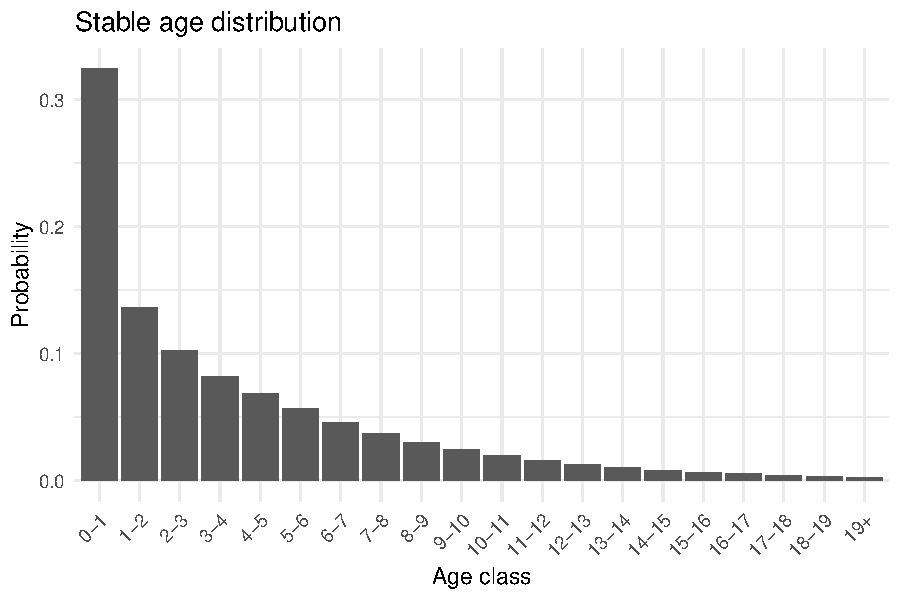
\includegraphics[width=0.8\textwidth]{../figures/age_distribution_p1.pdf}
	\caption{Latent age distribution $\boldsymbol{\pi}$ obtained from the normalized dominant eigenvector of the Leslie matrix $\mathbf{L}$.}
	\label{fig:stable_age}
\end{figure}

\subsection{Error term} \label{sec:error_terms}

In this section, we define the discretisation procedure used to construct the misclassification matrix $\textbf{M}$ described in Section \ref{par:measurement-error}. The chosen error model is designed to approximately reflect the error pattern shown in Figure 5(a) in \cite{nakamura2023}. 

For each individual with true age class $Z_r = j$, we assume an additive Gaussian measurement error as specified in \ref{par:measurement-error} with two distinct values of $\sigma$, namely $\sigma \in \{1,4\}$:
\[
\epsilon_r \mid Z_r \sim \mathcal{N}(0, \sigma^2).
\]

The observed value $j - 0.5 + \epsilon_r$ is discretised by assigning it to the corresponding age interval $[i-1,i)$.

To account for the lower boundary, we condition on the event that the perturbed value lies within the support of the age scale, resulting in a truncated distribution. The probability of observing class $i = 1,\dots,19$ is therefore
\[
M_{ij}
=
\frac{
	\Phi\!\left(\frac{i - (j - 0.5)}{\sigma}\right)
	-
	\Phi\!\left(\frac{i-1 - (j - 0.5)}{\sigma}\right)
}{
	1 - \Phi\!\left(\frac{0 - (j - 0.5)}{\sigma}\right)
}.
\]

For the upper boundary, the last age class absorbs all remaining probability mass:
\[
M_{20,j}
=
1 - \sum_{i=1}^{19} M_{ij}.
\]

This ensures that $\sum_{i=1}^{20} M_{ij} = 1$.

The resulting distribution corresponding to $\sigma = 4$ is shown in Figure~\ref{fig:stable_age_vs_D}.


\begin{figure}[H]
	\centering
	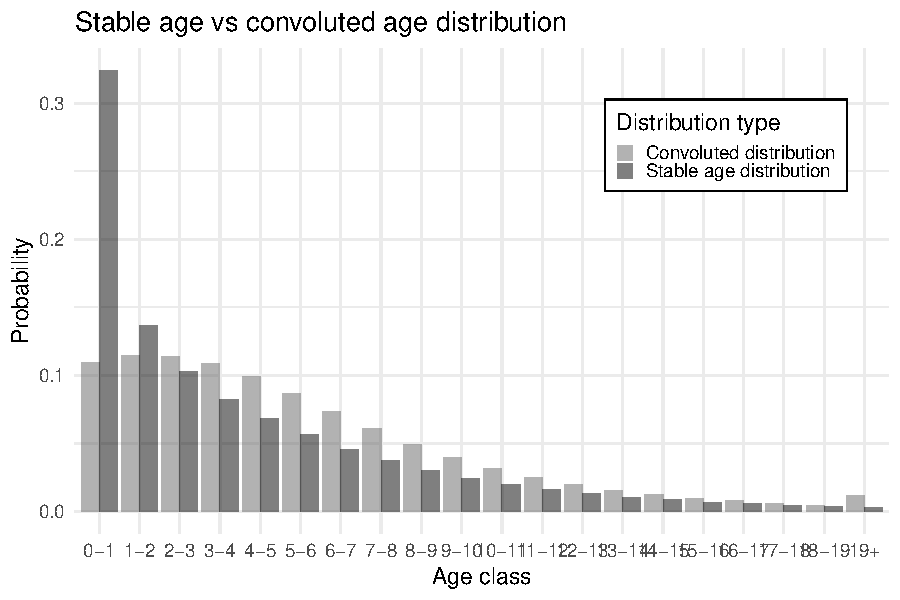
\includegraphics[width=0.8\textwidth]{../figures/age_distribution_comp_p2.pdf}
	\caption{Stable age distribution $\boldsymbol{\pi}$ and the corresponding observed age distribution $M\boldsymbol{\pi}$ under the measurement error model $\epsilon_r \mid Z_r \sim \mathcal{N}(0, 4^2)$.}
	\label{fig:stable_age_vs_D}
\end{figure}

\subsection{Simulation design}

This section describes the experimental setup used to evaluate the performance of the deconvolution methods.

The latent age distribution $\boldsymbol{\pi}$ is fixed across all simulations and corresponds to the stable age distribution derived from a Leslie matrix with $k = 20$ age classes (Section~\ref{sec:age_distribution}). Measurement error is introduced through a misclassification matrix $M$, constructed from the Gaussian error model described in Section~\ref{sec:error_terms} with two choices of $\sigma$, $\sigma = 1$ and $\sigma = 4$.

To study the effect of sample size, we consider
\[
n \in \{50, 100, 250, 1000\}.
\]

We compare four estimators of the latent distribution:
\begin{itemize}
	\item oracle estimator $\hat{\boldsymbol{\pi}_{oracle}} = \mathbf{Z}/n$
	\item the naive estimator $\hat{\boldsymbol{\pi}_{naive}} = \mathbf{Y}/n$,
	\item the method-of-moments estimator $\hat{\boldsymbol{\pi}}_{MoM}$,
	\item the EM-based maximum likelihood estimator $\hat{\boldsymbol{\pi}}_{ML}$ with naive initializator $\hat{\boldsymbol{\pi}}_{naive}$
\end{itemize}

For each configuration, the simulation is repeated $R = 1000$ times to assess variability and overall performance.

For the EM algorithm, convergence is declared when
\[
\ell(\boldsymbol{\pi}^{(t+1)}) - \ell(\boldsymbol{\pi}^{(t)}) < \epsilon,
\]
with $\epsilon = 10^{-4}$, or after a maximum of 1000 iterations.

The regularization parameter for the MoM estimator, $\lambda$, was chosen by visual inspection of Figure~\ref{fig:median_ci_dist}, selecting the smallest value that still produced a sufficiently smooth estimate. This resulted in $\lambda = 10^{-1}$ for $\sigma = 1$ and $\lambda = 10^{-2}$ for $\sigma = 4$.

\subsection{Simulation procedure}
\label{sec:simulation_procedure}

We evaluate the estimators using a Monte Carlo simulation. Each replication proceeds as follows:

\paragraph{Step 1: Generate latent data}
Sample age classes independently as
\[
\boldsymbol{Z} \sim \text{Multinomial}(n,\boldsymbol{\pi})
\]

\paragraph{Step 2: Apply measurement error}
For each individual with true age class $Z_r = j$, the observed class is sampled according to the misclassification probabilities:
\[
Y_r \mid Z_r = j \sim \text{Categorical}(M_{\cdot j}).
\]

\paragraph{Step 3: Estimate distribution}
Compute $\hat{\boldsymbol{\pi}}$ using each estimator.

\paragraph{Step 4: Evaluate performance}
Compute the total variation distance
\[
\mathrm{TV}(\hat{\boldsymbol{\pi}}, \boldsymbol{\pi})
= \frac{1}{2} \sum_{j=1}^{k} |\hat{\pi}_j - \pi_j|.
\]

\paragraph{Step 5: Forecasting analysis}
Forecasts based on $\hat{\boldsymbol{\pi}}$ are compared to those obtained from the true distribution $\boldsymbol{\pi}$ using the relative error in total population size defined in Section~\ref{sec:pop_model_matrix}.


\section{Results}
\subsection{Recovery of latent age distribution}


Overall, the simulation indicate that the EM maximum likelihood (ML) estimator provides the most accurate recovery of the latent age distribution in terms of diminished bias, but at the cost of increased variability. In contrast, the naive and MoM estimator is systematically biased, particularly in lower age classes, but exhibits substantially lower variability.

While the ML estimator better captures the expected structure of the latent distribution, its estimates are more sensitive to sampling variation and measurement error, especially in higher age classes.

From Figures~\ref{fig:median_tv_dist_rec}, it can be observed that the naive estimator produces smoother and more regular age profiles across adjacent bins. In contrast, the ML estimator yields more irregular patterns, with greater local fluctuations between neighbouring age classes, while the MoM estimator produces comparatively smooth but biased estimates. This behaviour is consistently observed across simulation replications and is not specific to this individual realisation of the estiamte.

\begin{figure}[H]
	\centering
	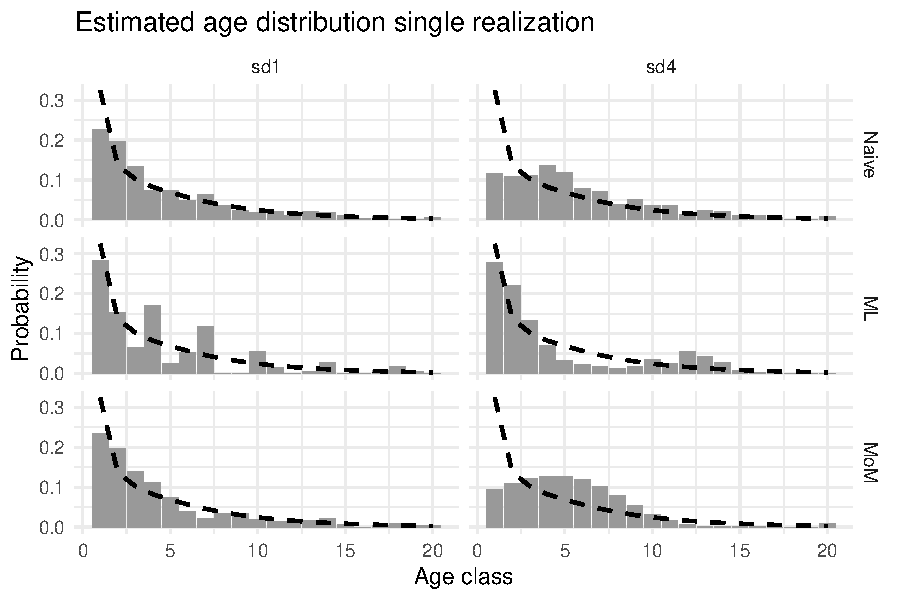
\includegraphics[width=0.8\textwidth]{../figures/estimate_median_distribution.pdf}
	\caption{
		Recovered latent age distributions for $n = 500$ using the ML, method-of-moments (MoM), and naive estimators under noise levels $\sigma = 1$ and $\sigma = 4$. 
		The displayed distribution corresponds to a single reconstruction, selected as the one whose total variation (TV) distance to the true latent distribution is closest to the median across all 1000 Monte Carlo simulations. 
		The dashed line represents the true latent age distribution.}
	\label{fig:median_tv_dist_rec}
\end{figure}

The singular estimate in Figure~\ref{fig:median_tv_dist_rec}, while informative, do not reflect the overall performance of the recovery methods. In Figure~\ref{fig:median_ci_dist}, we therefore present the median recovered age distribution across all simulations, together with the corresponding 2.5\% and 97.5\% Monte Carlo percentile bands based on 1000 replications.

Consistent with the previous figure, the naive estimator systematically underestimates lower age classes (0--3 years), with a more pronounced effect under higher noise ($\sigma = 4$). It can also be observed that the corresponding confidence bands for naive and MoM are considerably narrower than those of the ML estimator across all age classes.

The ML estimator exhibits a close fit to the true latent age distribution in terms of the median, but shows substantially higher variability compared to the naive estimator. This variability also becomes less smooth under the higher noise setting ($\sigma = 4$).

The MoM estimator displays a low variability high bias with additional mass being shifted toward higher age classes under ($\sigma = 4$). 

\begin{figure}[H]
	\centering
	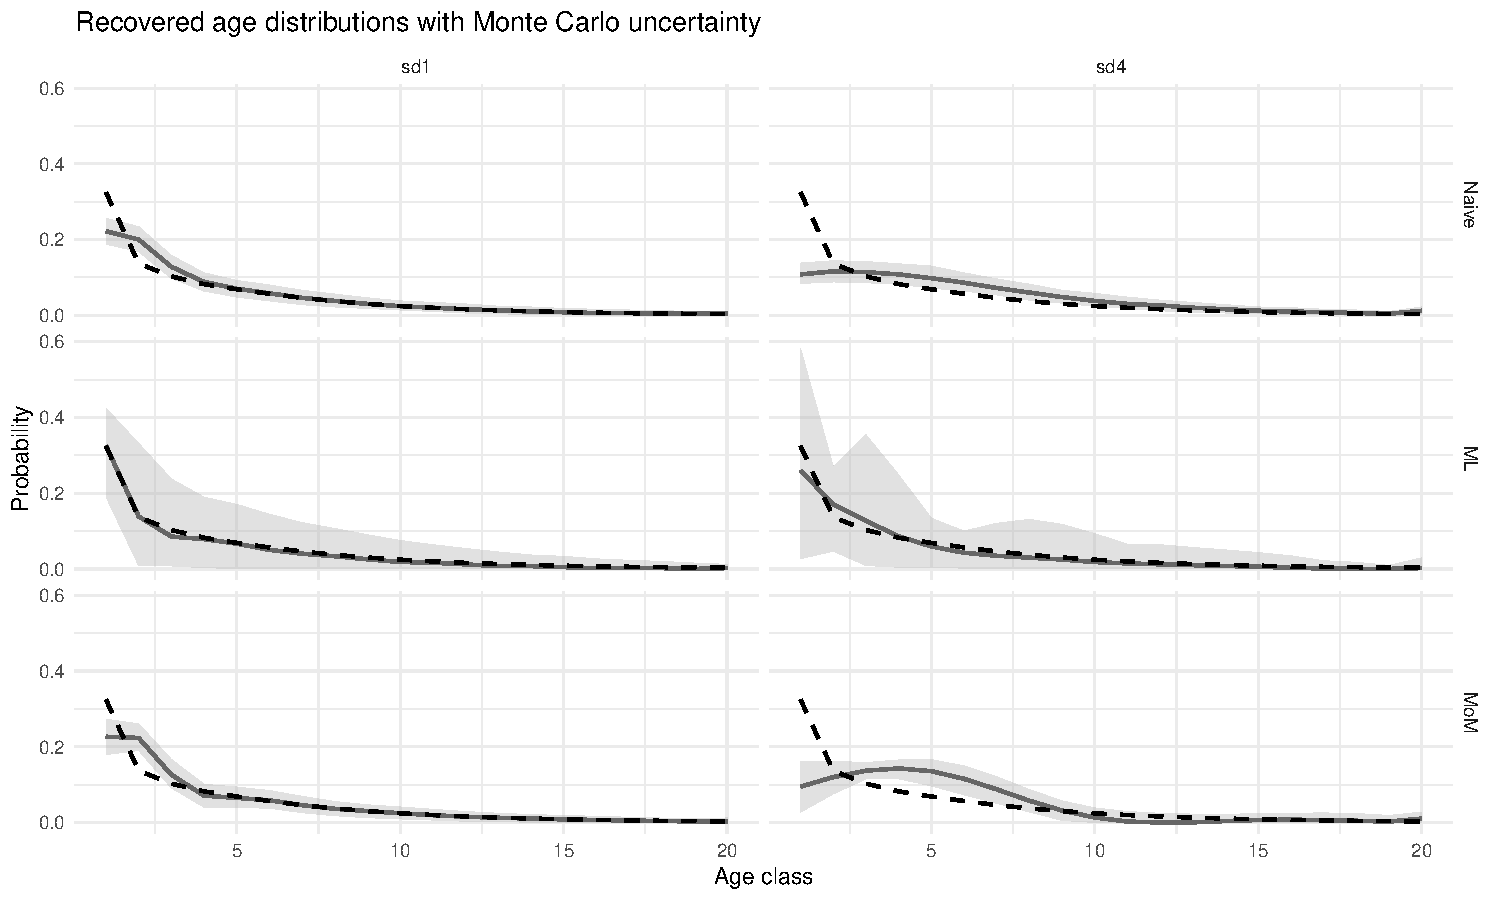
\includegraphics[width=0.8\textwidth]{../figures/confidence_interval_dist.pdf}
	\caption{Recovered latent age distributions for $n = 500$ using the ML, method-of-moments (MoM), and naive estimators under noise levels $\sigma = 1$ and $\sigma = 4$. 
		For each setting, the median estimate across 1000 Monte Carlo simulations is shown, with shaded regions indicating the 2.5\% and 97.5\% Monte Carlo percentiles. 
		The dashed line represents the true latent age distribution.}
	\label{fig:median_ci_dist}
\end{figure}

\subsection{Sample size effect on TV}

Having characterized the recovered distributions and their variability, we next quantify how estimator performance changes with sample size using total variation (TV) distance.

In Figure~\ref{fig:tv_vs_sample_size}, we observe how sample size affects the total variation (TV) distance across estimators. The method of moments (MoM) estimator exhibits a slightly higher TV distance across both noise settings relative to the naive estimator, with little sensitivity to sample size.

The naive estimator tracks the oracle baseline more closely than the ML and MoM estimators in both noise settings except for $\sigma = 4$ and $n > 500$. 

The maximum likelihood (ML) estimator shows consistent improvement with increasing sample size in both error settings, with a higher baseline TV distance under $\sigma = 4$ than under $\sigma = 1$. Among all estimators, ML exhibits the strongest negative dependence with increased sample size within the considered range, and this trend does not appear to taper off.

\begin{figure}[H]
	\centering
	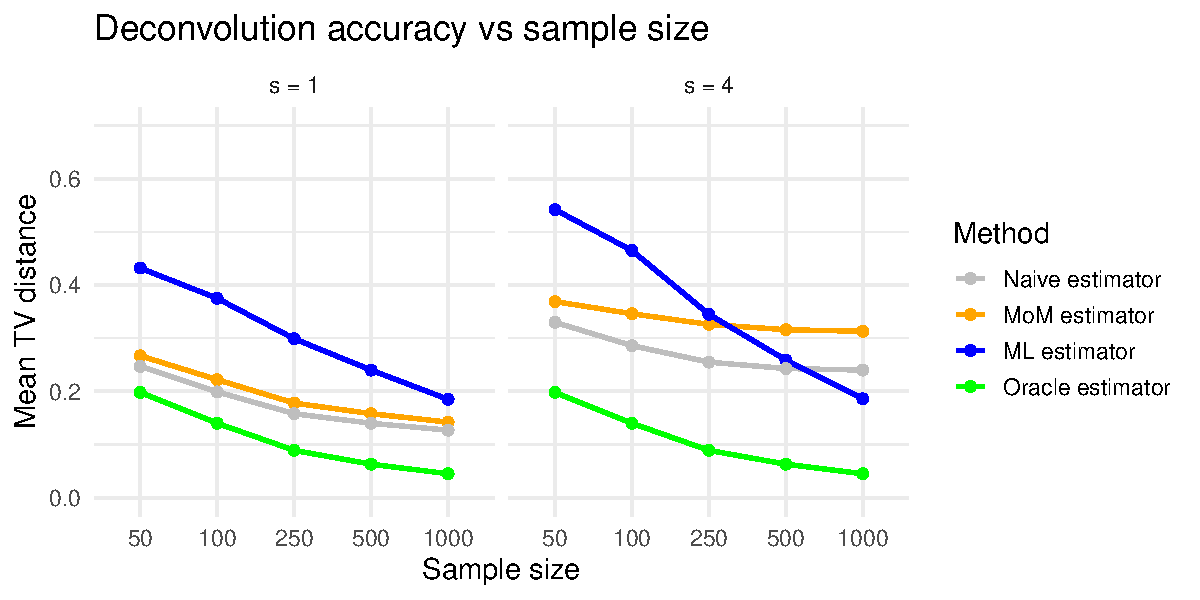
\includegraphics[width=0.8\textwidth]{../figures/lineplot_sz_decon.pdf}
	\caption{
			Mean total variation (TV) distance between estimated $\hat{\boldsymbol{\pi}}$ and true age distribution $\boldsymbol{\pi}$ across five sample sizes, based on 1000 Monte Carlo replications. Results are shown for four estimators: the naive estimator, method of moments (MoM), EM-based maximum likelihood (EM), and an oracle baseline obtained by sampling directly from the true latent distribution $\boldsymbol{\pi}$. Panels correspond to different measurement error levels ($\sigma = 1$ and $\sigma = 4$).}
	\label{fig:tv_vs_sample_size}
\end{figure}

To isolate the effect of sampling variability on the total variation (TV) distance, we adjust the observed TV distances by subtracting the corresponding TV distance obtained from the oracle baseline. Consistent with Figure~\ref{fig:tv_vs_sample_size}, the maximum likelihood (ML) estimator exhibits a strong dependence on sample size, with the TV distance decreasing as sample size increases. In contrast, both the MoM and naive estimators show increasing TV distance with sample size.

\begin{figure}[H]
	\centering
	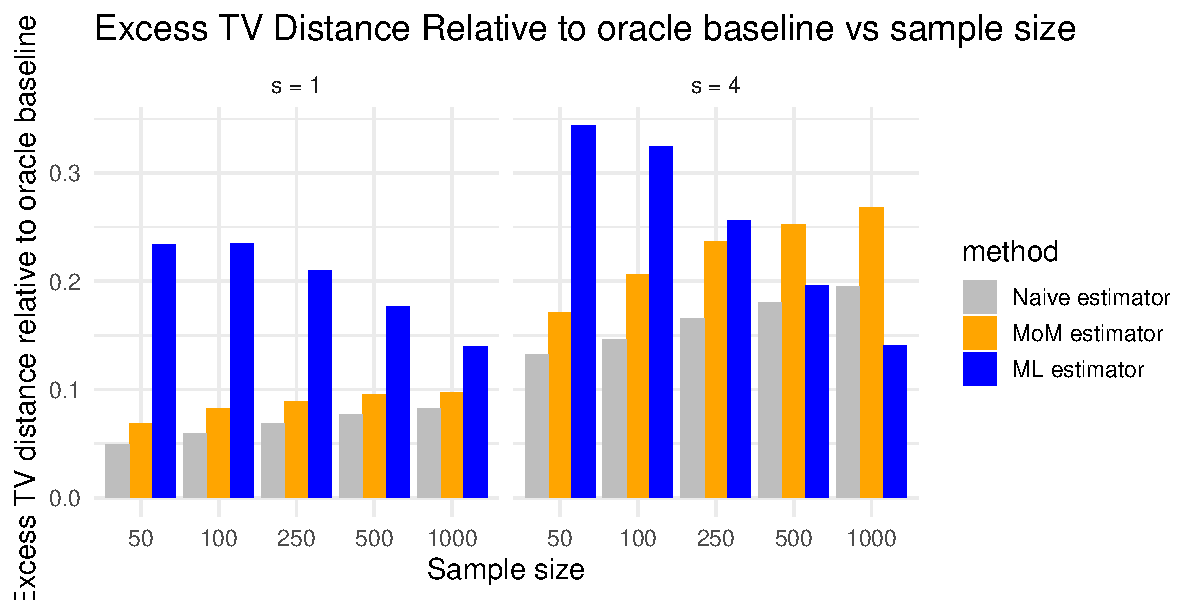
\includegraphics[width=0.8\textwidth]{../figures/barplot_c_MoM_i_TV_minus_baseline_p8.pdf}
	\caption{
		Mean excess total variation (TV) distance relative to the oracle baseline across sample sizes and estimation methods, based on 1000 Monte Carlo simulations. The excess TV is defined as
		$\mathrm{TV}(\hat{\boldsymbol{\pi}}, \boldsymbol{\pi}) - \mathrm{TV}(\hat{\boldsymbol{\pi}}_{\mathrm{oracle}}, \boldsymbol{\pi})$.}
	\label{fig:dif_tv_rel_oracle}
\end{figure}

We now proceed to examine the distribution and variability in total variation (TV) distance across estimators. The previous plots have focused on mean performance, whereas the violin plot in Figure~\ref{fig:violin_TV} illustrates the full distribution of TV distances across Monte Carlo replications. 

The results show that the TV distance for the naive and MoM estimators is more tightly concentrated around their respective medians, with the MoM estimator exhibiting slightly higher variability. In contrast, the ML estimator displays a substantially wider distribution of TV distances. This spread becomes more pronounced for both the MoM and ML estimators under the higher noise level $\sigma = 4$.

\begin{figure}[H]
	\centering
	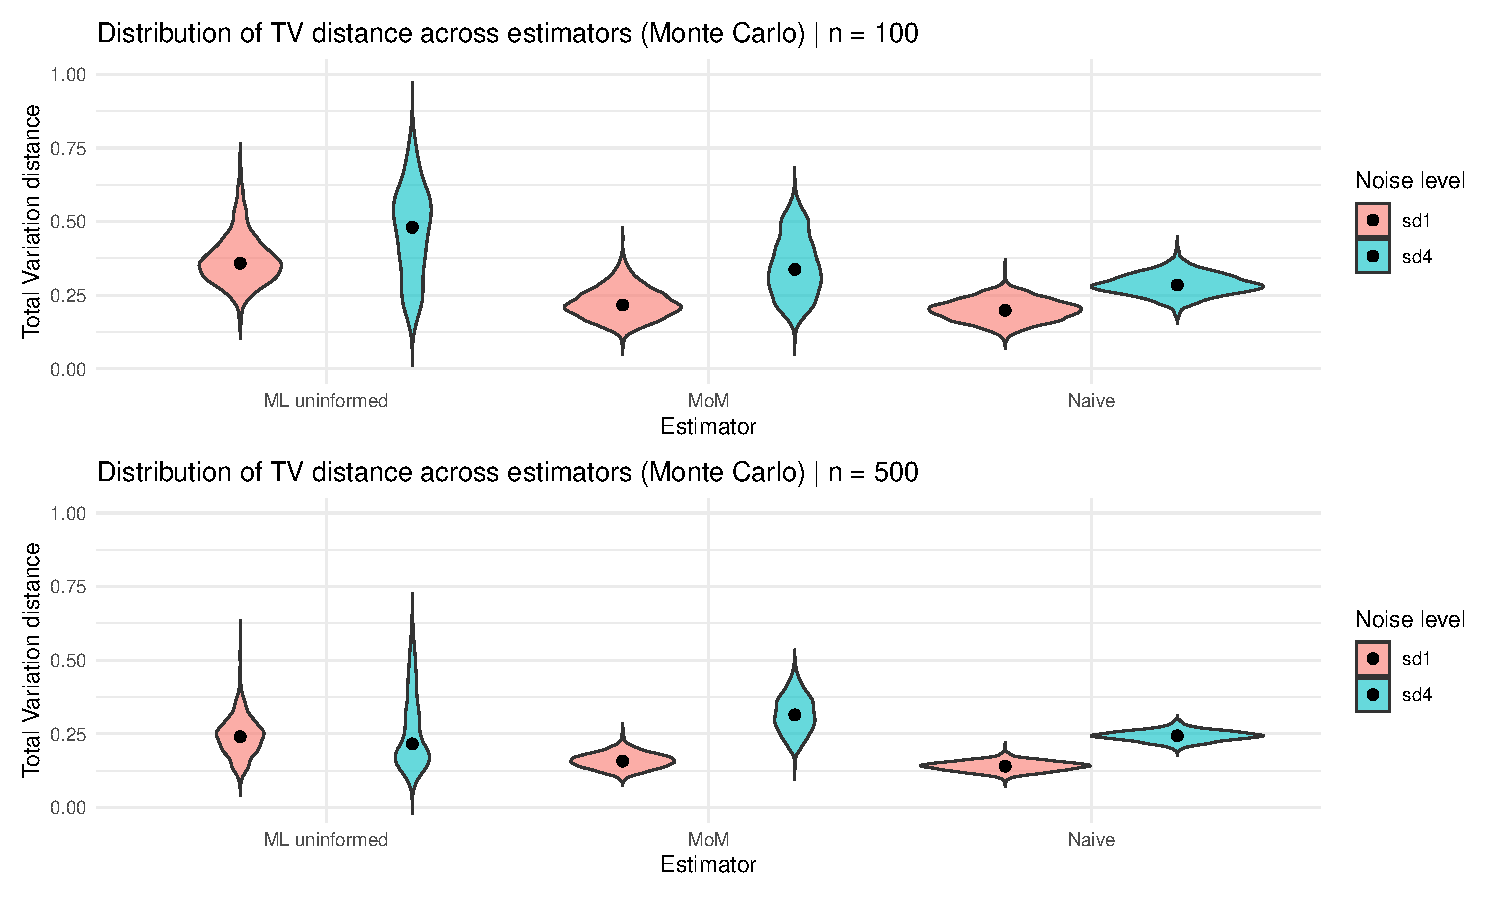
\includegraphics[width=0.8\textwidth]{../figures/violin.pdf}
	\caption{
		Violin plot of total variation (TV) distance across 1000 Monte Carlo replications for three estimators under noise levels $\sigma = 1$ and $\sigma = 4$. The upper panel corresponds to sample size $n = 100$, while the lower panel corresponds to $n = 500$.
	}
	\label{fig:violin_TV}
\end{figure}


\subsection{Population forecast}

As mentioned in Section~\ref{sec:Leslie_Matrix}, population dynamics are governed by the Leslie matrix framework. We evaluate how estimation errors in the initial age distribution propagate into five-year total population forecasts.

Figure~\ref{fig:tp_forecast} shows the deviation of estimated total population sizes from the true latent population. A mean value close to zero indicates an unbiased population forecast.

The naive estimator exhibits a smaller bias when $\sigma = 1$ compared to $\sigma = 4$, corresponding to approximately 16\% and 76\% higher total population at year five, respectively. Overall, the naive estimator shows relatively low variability compared to the other estimators.

The MoM estimator exhibits slightly lower variability than the ML projection but shows a positive bias, consistently overestimating the total population by approximately 10\% for $\sigma = 1$ and 59\% for $\sigma = 4$.

The EM-based ML estimator appears approximately unbiased in terms of its expected total population forecast, but exhibits substantially higher uncertainty compared to the naive estimator.

\begin{figure}[H]
	\centering
	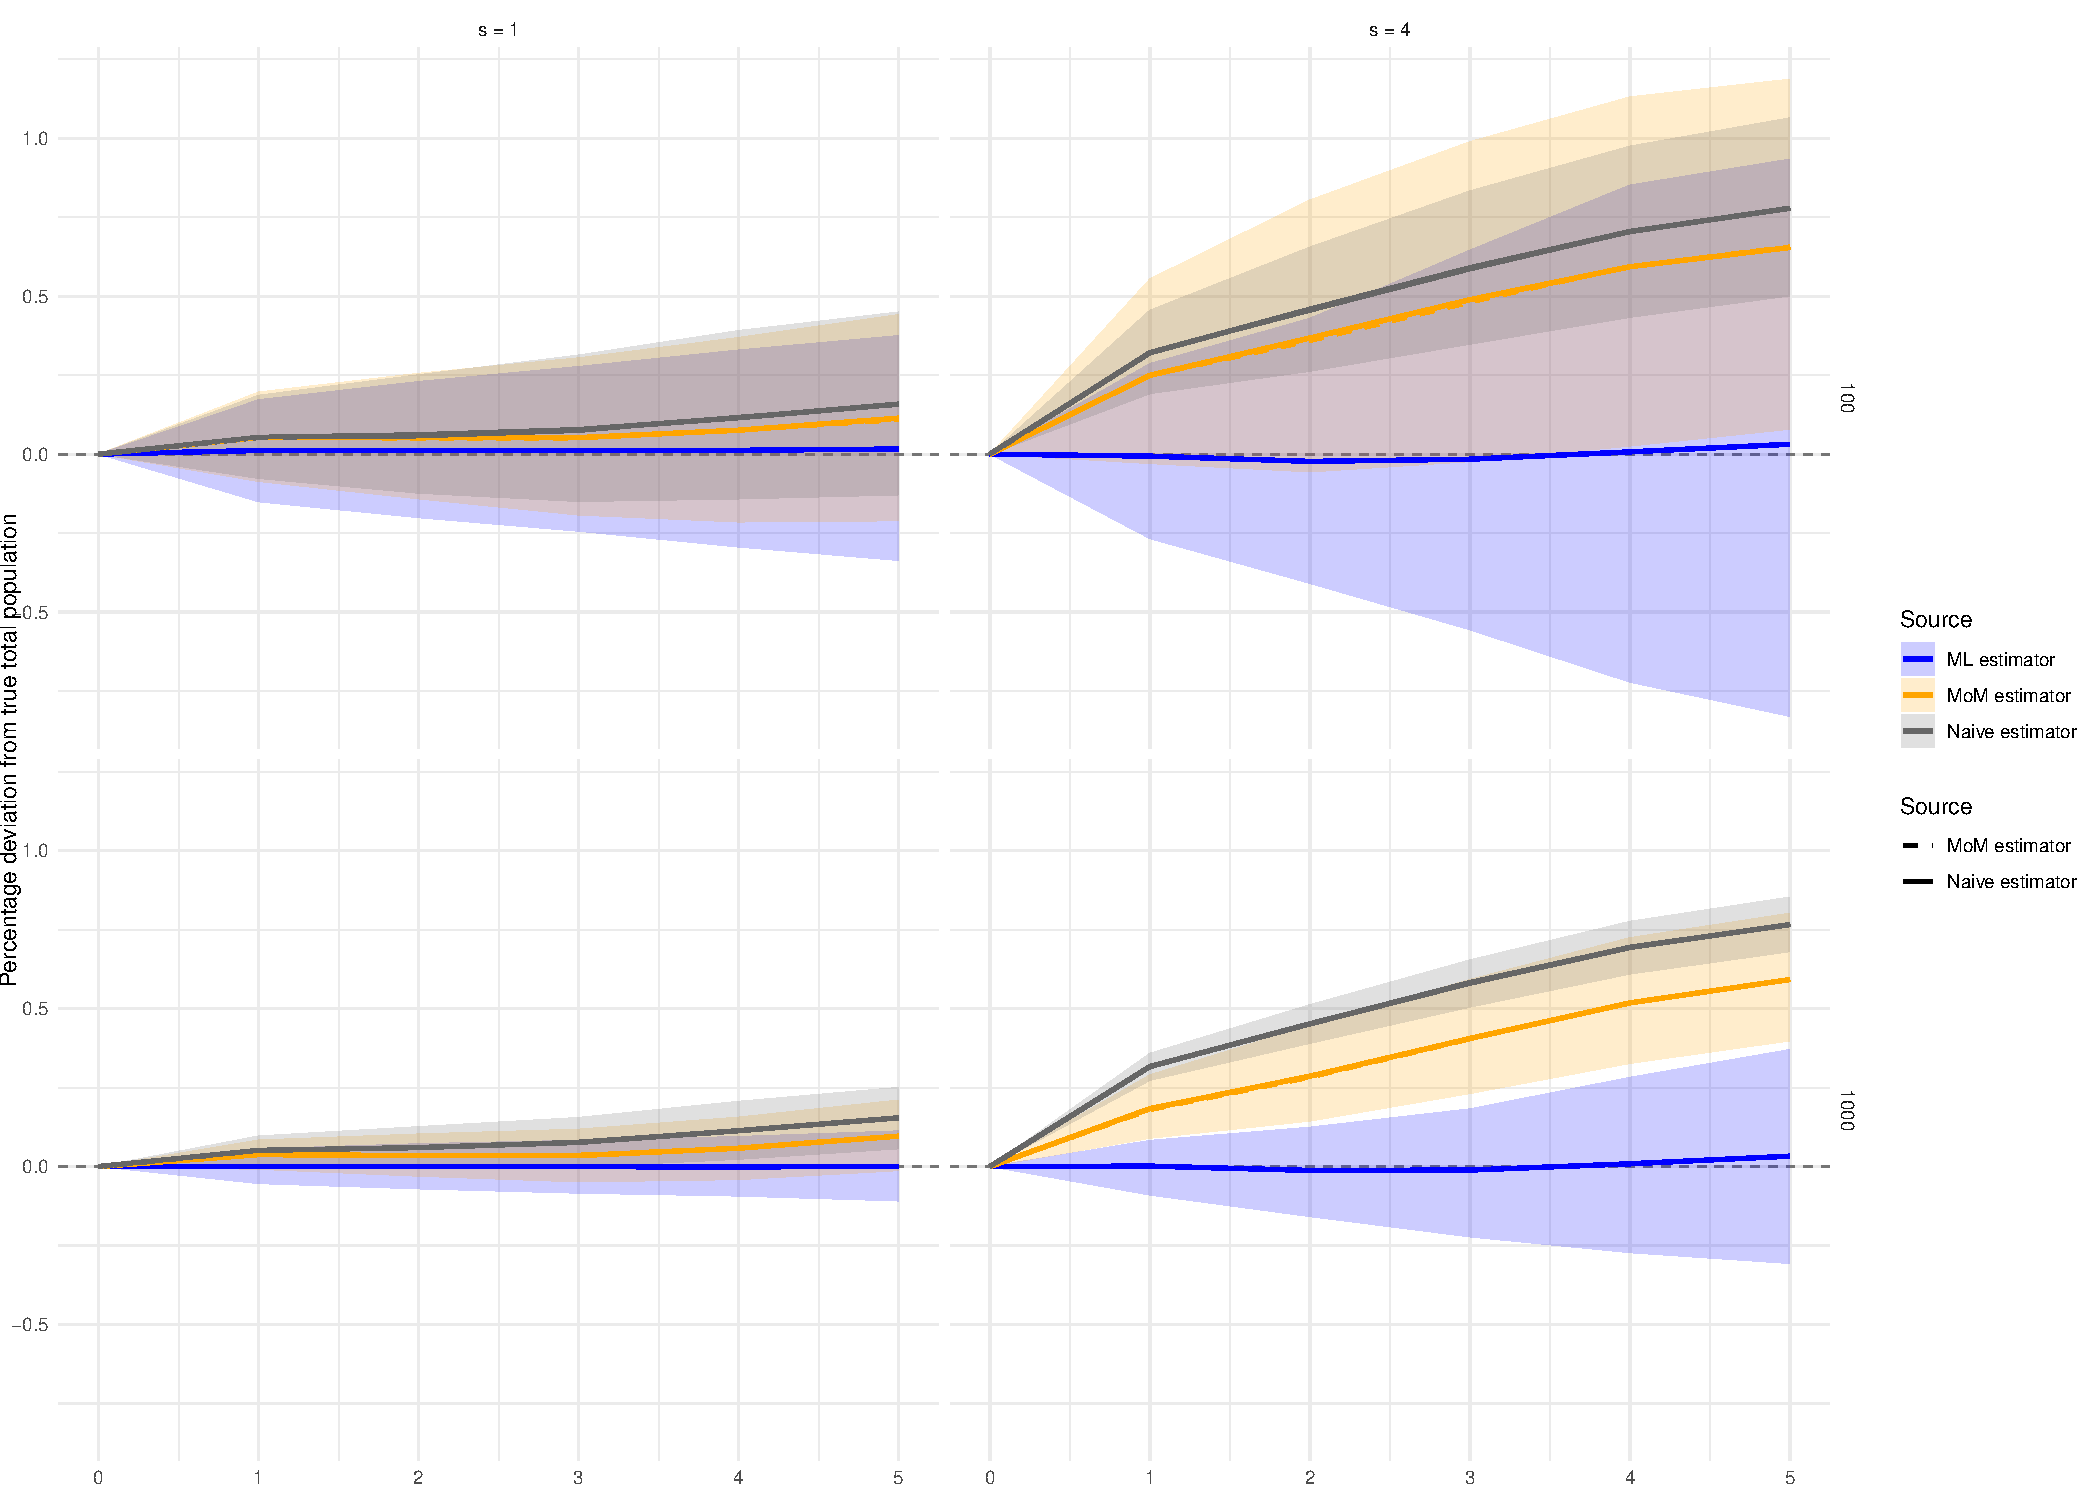
\includegraphics[width=0.8\textwidth]{../figures/forcast_plot.pdf}
	\caption{
			Five-year population forecast error under different estimators and measurement error levels ($\sigma = 1$ and $\sigma = 4$), based on 1000 Monte Carlo simulations. The forecasts are obtained by propagating the estimated initial age distributions $\hat{\boldsymbol{\pi}}$ through the Leslie matrix dynamics defined in \ref{subsub:forcast}. Results are shown for the naive estimator, method-of-moments (MoM), and EM-based maximum likelihood (ML) estimator with sample size 100 and 1000.
	}
	\label{fig:tp_forecast}
\end{figure}








\section{Analysis / Discussion}

The results of this simulation study show that the latent age distribution can be recovered with a less biased estimate using the EM-based maximum likelihood estimator, but at the cost of increased variability under both low ($\sigma = 1$) and high ($\sigma = 4$) measurement error. In contrast, the naive estimator and MoM estimator yielded a biased but smoother age distribution. Systematically underestimates the proportion of younger individuals (ages $< 3$ years), which results in a corresponding overestimation of older age classes.

Although this bias may appear small in magnitude, its impact is non-negligible in the context of population forecasting. Shifts in probability mass away from demographically critical age classes, especially those contributing most to reproduction, can lead to disproportionately large errors in projected population size. This highlights that even modest bias in age structure estimates can have substantial downstream consequences when used in population models. 

\subsection{Properties of estimators}

As expected from Figure~\ref{fig:stable_age_vs_D}, the naive estimator produces biased estimates due to the misclassification matrix $M$. This bias becomes more pronounced as the sample size increases, as illustrated in Figure~\ref{fig:dif_tv_rel_oracle}.

For small sample sizes, the total variation (TV) distance of the naive estimator is largely dominated by sampling variability. As a result, the difference between the naive estimator and the oracle baseline is relatively small. However, as the sample size increases, the effect of sampling variability diminishes, and the remaining error is primarily driven by the systematic bias introduced by the misclassification process.

Formally, by the law of large numbers and the continuous mapping theorem (see p.~356 in \cite{robert2007}), we have that as $n \to \infty$:
\[
\mathrm{TV}(\hat{\boldsymbol{\pi}}_{\text{oracle}}, \boldsymbol{\pi}) \to 0,
\]
while the naive estimator converges to the biased distribution $M\boldsymbol{\pi}$, such that
\[
\mathrm{TV}(\hat{\boldsymbol{\pi}}_{naive}, \boldsymbol{\pi}) \to \mathrm{TV}(M\boldsymbol{\pi}, \boldsymbol{\pi}).
\]
This explains the increase in TV with sample size for the naive estimator in Figure~\ref{fig:dif_tv_rel_oracle}.

Similarly to the naive estimator the MoM would roughly converge wtih $n \to \infty$ to:

\begin{equation}
\mathrm{TV}(\hat{\boldsymbol{\pi}}_{\mathrm{MoM}}, \boldsymbol{\pi})
\to
\mathrm{TV}(A_\lambda \boldsymbol{\pi}, \boldsymbol{\pi})
\label{eq:conv_tv_mom}
\end{equation} 

The method-of-moments (MoM) estimator is limited in its recovery of the latent age distribution by the instability of matrix inversion. Matrix inversion does not guarantee constraints such as non-negative probabilities or summing to one, which is accounted for by truncation to 0 and renormalisation. This projection violates the assumptions of the continuous mapping theorem; thus, we do not expect exact convergence to equation \eqref{eq:conv_tv_mom}. The MoM is therefore limited in its recovery of the latent age distribution by this bias.

The EM maximum likelihood (ML) estimator, as mentioned in the results, exhibited a decreasing TV distance with sample size relative to the oracle baseline \ref{fig:dif_tv_rel_oracle}. However, it shows a significantly larger spread in its TV distribution as showcased in \ref{fig:violin_TV}. The overall smooth shape of the violin plot (no clear clusters) for TV suggests that the EM algorithm is not converging to distinct local maxima or plateaus, but rather operates in a relatively flat log-likelihood surface, supported by the convergence diagnostics \ref{app:failure_rate} indicating that the maximum number of iterations is usually not reached. This is symptomatic of an ill-posed EM deconvolution problem, where weak identifiability leads to or unstable convergence behaviour. Which seems adjustable by increased sample size. 

The EM maximum likelihood (ML) estimator, as shown in the results, exhibits a decreasing TV distance with increasing sample size relative to the oracle baseline \ref{fig:dif_tv_rel_oracle}. However, it shows a significantly larger spread in its TV distribution, as illustrated in Figure~\ref{fig:violin_TV}. The overall smooth shape of the violin plot, with no clear clustering, suggests that the EM algorithm does not converge to distinct local maxima or plateaus. Instead, it appears to operate on a relatively flat log-likelihood surface, consistent with the convergence diagnostics in \ref{app:failure_rate}, which shows that the maximum number of iterations is rarely reached. 

This behaviour is characteristic of an ill-posed deconvolution problem, where weak identifiability leads to unstable convergence behaviour. The results suggest that this instability is partially mitigated as sample size increases.

We identify in this simulation study that deconvolution through EM maximum likelihood and method-of-moments (MoM) exhibit different failure modes. While the MoM estimator is affected by numerical instability due to inversion of near-singular matrices, as well as the lack of enforced probability constraints (non-negativity and unit sum), the EM algorithm instead suffers from poor identifiability, reflected in a relatively flat log-likelihood surface. In the MoM case, this leads to unstable and often non-admissible estimates unless regularized, whereas for EM the main issue is not feasibility but sensitivity to the observed data and slow movement through a weakly identified parameter space. This distinction highlights that both methods are affected by the ill-posed nature of the deconvolution problem, but in fundamentally different ways: MoM through numerical instability, and EM through weak identifiability and flat likelihood.

\subsection{Practical Implications}

The results above have focused on statistical properties and estimator behaviour. We now turn to the practical motivation for estimating age distributions and evaluate how the different estimators affect total population forecasts in an ecological context.

As shown in Figure \ref{fig:tp_forecast}, both MoM and ML outperform the naive estimator in terms of mean and median under both high and low noise, as well as for small and large sample sizes. In particular, we observe that MoM exhibits a slightly wider Monte Carlo percentile band in \ref{fig:median_ci_dist}, closer to that of the naive estimator, but with a differently skewed bias.

This suggests that for ecological indicators such as these, the direction and structure of the bias may be more important than its magnitude alone. Specifically we know from \label{app:leslie_params} that miscclasifying individuals of fertile >4 years to none fertile ages < 4 or viceversa will significantly alter the forcast. This is consistent with our expected meassurment error \ref{fig:stable_age_vs_D} thus leading to the naive estimator overestimating individuals of fertile age. 

Whether the MoM or ML estimator is preferable over the naive estimator therefore depends on the decision-maker?s tolerance for variability, the forecast horizon, and constraints related to sampling cost and sample size.

\subsection{Viability of assumptions \& improvements}

In order to study the deconvolution methods in a controlled setting, several simplifying assumptions were made. The misclassification matrix $M$ was assumed to be fully known. In practical applications, however, $M$ must typically be estimated from auxiliary data panel 5 fig a \ref{ref:}, introducing additional uncertainty. The results presented in this study should therefore be interpreted with caution, as they represent a best-case scenario for deconvolution performance.

Regarding the method-of-moments estimator, the choice of regularization parameter $\lambda$ was based on visual inspection and is therefore unlikely to be optimal. A more objective approach, such as cross-validation or other data-driven selection criteria, would provide a more appropriate level of regularization and yield a fairer comparison between estimators.

For the EM algorithm, the use of multiple initialization points per sample or the inclusion of additional constraints in the maximization step could improve stability and robustness. In particular, initialization based on the naive estimator may result in zero-valued components, which prevents recovery of those classes in subsequent iterations \ref{eq:maximization_setp}. This highlights the sensitivity of the EM algorithm to initialization in this setting.

Finally, the population forecasting analysis assumes a fixed Leslie matrix $\mathbf{L}$ and a stable age distribution. In realistic ecological settings, demographic parameters such as fertility and survival vary over time and must themselves be estimated from data, introducing additional sources of uncertainty. It is therefore plausible that, in practice, the combined effect of these uncertainties may dominate the forecasting error, potentially reducing the impact of improvements obtained through deconvolution.

Overall, this thesis provides insight into the behaviour of different estimators under simplified and controlled conditions in an ill-posed deconvolution setting, as well as demonstrating a practical use case and its implications in an applied ecological context.
 



\section{Appendix}

\label{app:leslie_params}

\begin{table}[ht]
	\centering
	\caption{Parameters used to construct the Leslie matrix.}
	\label{tab:leslie_params}
\begin{tabular}{rrrrr}
	\hline
	Age & Survival & p\_coy & Litter\_size & F\_i \\ 
	\hline
	1 & 0.50 & 0.00 & 0.00 & 0.00 \\ 
	2 & 0.89 & 0.00 & 0.00 & 0.00 \\ 
	3 & 0.95 & 0.00 & 0.00 & 0.00 \\ 
	4 & 0.99 & 0.00 & 0.00 & 0.00 \\ 
	5 & 0.98 & 0.15 & 2.12 & 0.31 \\ 
	6 & 0.96 & 0.35 & 2.25 & 0.76 \\ 
	7 & 0.96 & 0.55 & 2.40 & 1.27 \\ 
	8 & 0.96 & 0.55 & 2.40 & 1.27 \\ 
	9 & 0.96 & 0.55 & 2.40 & 1.27 \\ 
	10 & 0.96 & 0.55 & 2.40 & 1.27 \\ 
	11 & 0.96 & 0.55 & 2.40 & 1.27 \\ 
	12 & 0.96 & 0.70 & 2.60 & 1.75 \\ 
	13 & 0.96 & 0.70 & 2.60 & 1.75 \\ 
	14 & 0.96 & 0.70 & 2.60 & 1.75 \\ 
	15 & 0.96 & 0.70 & 2.60 & 1.75 \\ 
	16 & 0.96 & 0.70 & 2.60 & 1.75 \\ 
	17 & 0.96 & 0.58 & 2.75 & 1.53 \\ 
	18 & 0.96 & 0.58 & 2.75 & 1.53 \\ 
	19 & 0.96 & 0.58 & 2.75 & 1.53 \\ 
	20 & 0.96 & 0.58 & 2.75 & 1.53 \\ 
	\hline
\end{tabular}
\end{table}

\begin{table}[H]
	\centering
	
\begin{tabular}{lrr}
\toprule
SD & SampleSize & FailureRate\\
\midrule
sd1 & 50 & 0.000\\
sd1 & 100 & 0.000\\
sd1 & 250 & 0.000\\
sd1 & 500 & 0.000\\
sd1 & 1000 & 0.000\\
\addlinespace
sd4 & 50 & 0.456\\
sd4 & 100 & 0.349\\
sd4 & 250 & 0.174\\
sd4 & 500 & 0.077\\
sd4 & 1000 & 0.022\\
\bottomrule
\end{tabular}

	\caption{
		Failure rate of the EM algorithm, defined as the proportion of Monte Carlo replications in which the algorithm did not converge within the maximum number of iterations.
	}
	\label{app:failure_rate}
\end{table}


\printbibliography

\end{document}   % H�r slutar dokumentet


\overset{d}{=}

